\section{Aufbau der Applikation}
\label{sec:Aufbau der Applikation}

\subsection{Einleitung}
Zur Entwicklung des \tool{}s wird wegen den im Kapitel Analyse erläuterten Gründen die Programmiersprache Go eingesetzt. Go erlaubt zwar einen Objekt-Orientierten Stil des Programmieren \cite[:240]{golang_faq}, bietet aber im Vergleich zu typisch \acs{OOP} Sprachen wie Java oder C++ keine Klassen \& Typen Hierarchie.

Anstatt von Klasse als Struktur bietet Go sogenannte Packages an. Innerhalb einer Package können beliebig viele \code{.go} Files erstellt werden, die dann den Source Code enthalten. Private Variablen und Funktionen sind innerhalb einer Package frei zugänglich, können aber ausserhalb der Package nicht aufgerufen werden.

\begin{lstlisting}[language=bash, caption=Package Struktur des \tool{}]                    
github.com/ipsecdigatool/ipsecdigatool/       
	.git/
	capture/ # Pakete von Netzwerkadapter capturen        
		capture.go
	config/ # Konfiguration erstellen, laden, aktualisieren
		config.go
	logging/ # Syslog Nachrichten absetzen
		logging.go
	mtu/ # MTU Discovery durchfuehren
		analyze.go
		capture.go
		send.go
	packetloss/ # Packet loss feststellen
		detect.go
		espmap.go
		lostfile.go
	main.go # Programmstart und Daemon Funktionalitaet
\end{lstlisting}

Die Packages \code{capture}, \code{config}, \code{logging} werden sowohl für die \acs{MTU} Discovery als auch für die Packet Loss Detection verwendet. Die Packages \code{mtu} und \code{packetloss} werden nur für die jeweiligen Funktionen gebraucht und sind unabhängig voneinander. Das \code{main.go} enthält allen Code der für den Programmstart sowie den Daemon Mode gebraucht wird.

\subsection{Namenskonvention}
Go unterscheidet öffentliche und private Funktionen und Variablen durch die Grosse- oder Kleinschreibung des ersten Buchstaben eines Funktions- oder Variablennamens. Gross geschriebene Namen zeigen eine öffentliche Funktion oder Variable an, die dann auch ausserhalb der Package genutzt werden kann.
In der Go Usergroup ist ausserdem auch die Idee verbreitet, dass Variablen- und Funktionsnamen möglichst kurz und prägnant sein sollen. CamelCase Namen sollen nach Möglichkeit vermieden werden. Dies kommt wohl einerseits von der C-Ähnlichkeit hat aber andererseits auch einen praktischen Grund. So ist ein Funktionsaufruf wie \code{capture.Start()} tatsächlich recht elegant und gut verständlich.
Im Verlauf dieses Projekts haben wir auch festgestellt, dass es besser ist alle Namen, Ordnernamen und Kommandos wenn möglich klein zu schreiben. Zu Beginn des Projekts haben wir \code{github.com/IPsecDiagTool/IPsecDiagTool} als Repository Ordner Struktur verwendet und dies hat zu einigen Konflikten geführt. Glücklicherweise lassen sich Repositories auf github.com relativ leicht umbenennen und wir konnten auf eine rein klein geschriebene Ordner Struktur umsteigen.

\subsection{Programmstart \& Multi-Threading}
Am Programmstart des \tool{} lässt sich das Zusammenspiel der verschiedenen Packages beobachten. Zuerst wird jeweils die Konfiguration geladen. Falls kein Konfigurationsfile auf dem System vorhanden ist wird ein neues File mit Default Werten erstellt. Danach werden die \code{logging} und \code{mtu} Packages initialisiert.

\begin{figure}[ht]
    \begin{center}
    % GFX Trim left bottom right top
        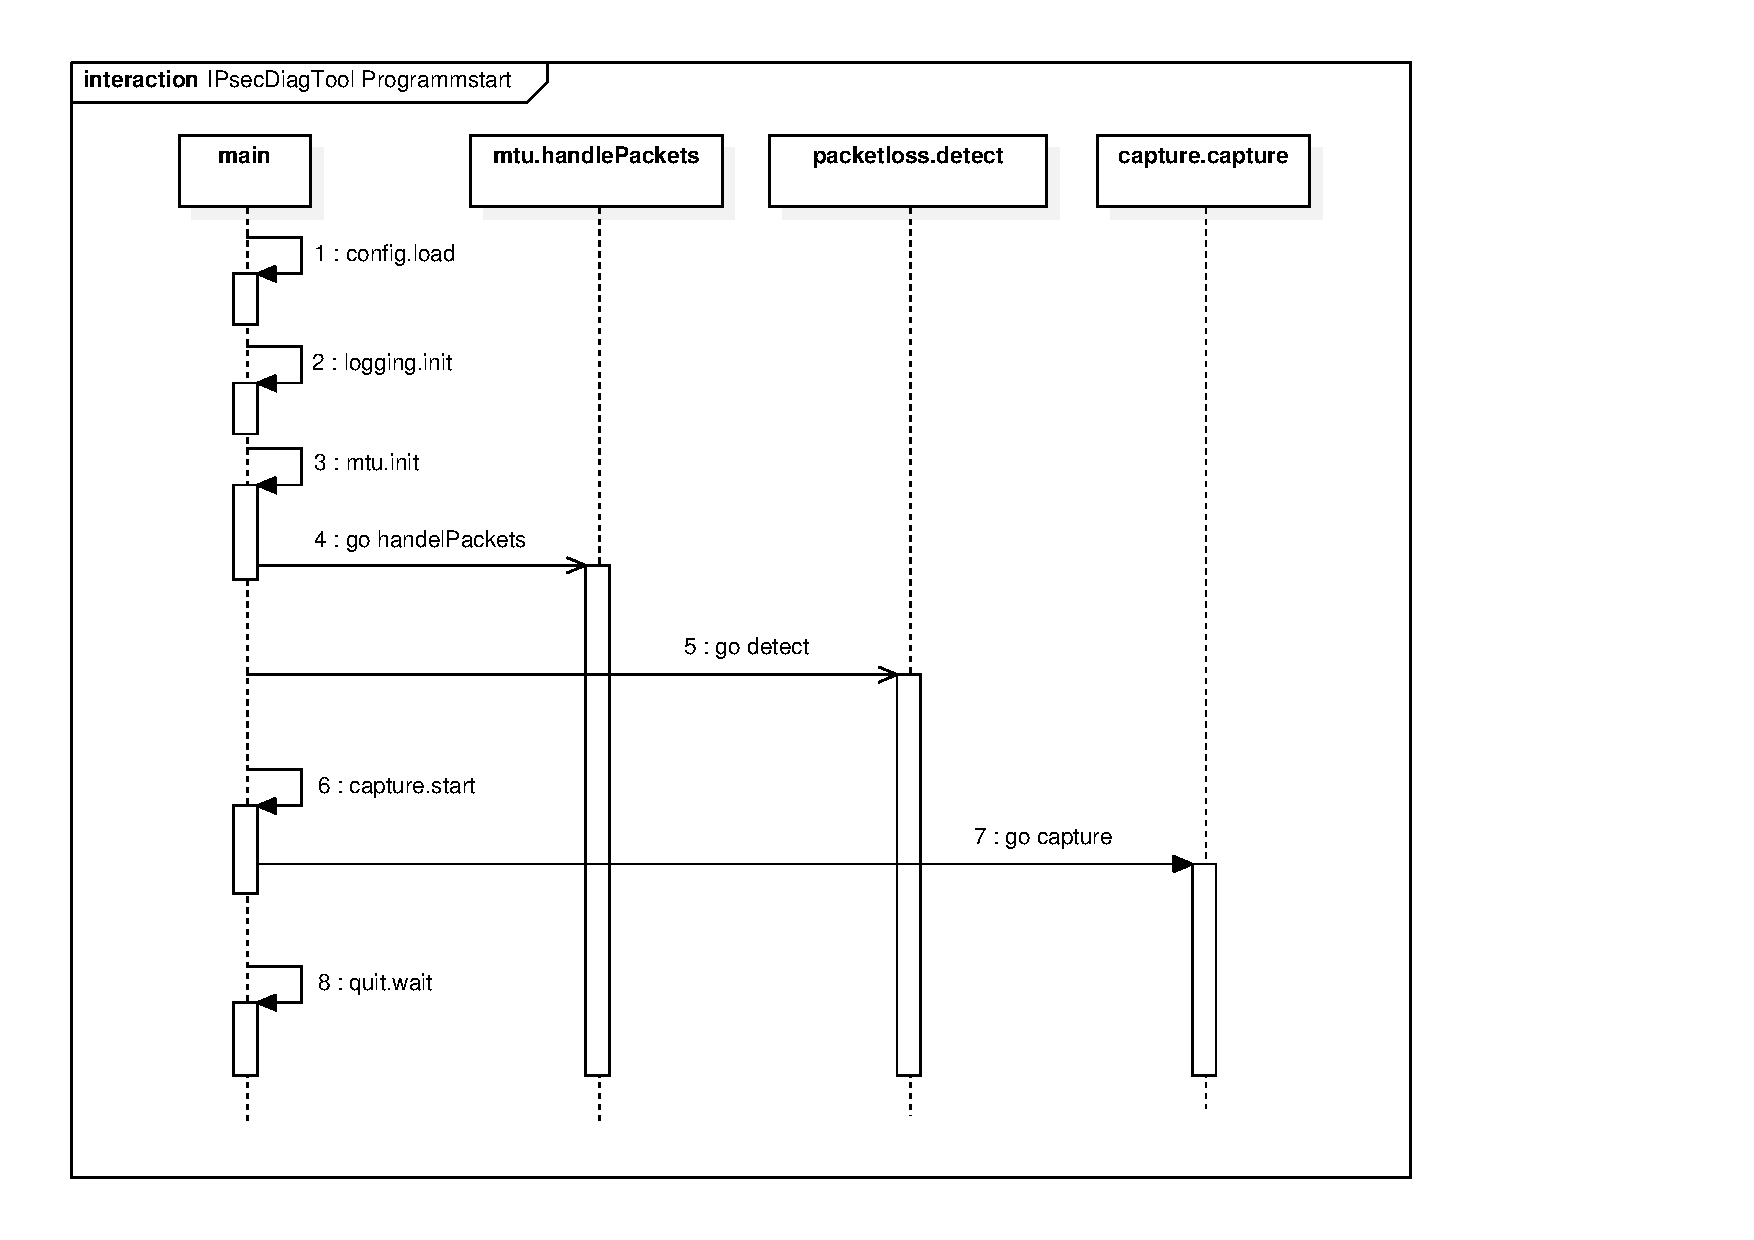
\includegraphics[trim=30 20 150 30,clip,width=\textwidth]{mainpart/implementation/img/programmstart}
    \end{center}
    \caption{Programmstart des \tool{}}
\end{figure}

Beim Initialiserungs-Vorgang der jeweiligen Package werden die für das Multi-Threading notwendigen Konstrukte erstellt. Bei Go wird Multi-Threading vor allem via Goroutinen und Channels realisiert. Eine Goroutine ist eine Funktion die im gleichen Address Space, gleichzeitig mit anderen Goroutinen ausgeführt wird. Goroutinen sind leichtgewichtig und kosten bei der Erstellung nicht mehr als Stack Space. Um Nebenläufigkeit zu erreichen, werden Goroutinen auf mehrere Threads des Betriebsystems multiplexed. Wenn eine Goroutine blockiert, können die anderen Goroutinen weiterlaufen \cite[:1391]{effective_go}.
Zur Synchronisation und zum Datenaustausch zwischen Goroutinen werden sogenannte Channels verwendet. Typischerweise hat man in einer Goroutine eine for-Schleife und wartet darin auf Input aus einem Channel.

Nachdem Initialisieren werden die Goroutinen der \code{mtu} und \code{packetloss} Packages gestartet. Zum Schluss wird die \code{capture} Goroutine gestartet. Ab jetzt werden die Pakete vom konfigurierten Interface aufgezeichnet und vom \tool{} verarbeitet. Die Main Funktion ist nur noch dafür verantwortlich ein vom User gesendetes \code{SIGTERM} Signal abzufangen und gegebenenfalls das Programm zu beenden.

\subsection{Pakete einfangen}
Das Einfangen von Paketen mit \ac{PCAP} ist in der \code{capture} Package implementiert. Sie bietet nur eine öffentliche Funktion die via \code{capture.Start(..)} aufgerufen werden kann. Als Parameter nimmt die Funktion die Konfiguration sowie ein Channel für \ac{ICMP}s und ein Channel für \ac{ESP}s entgegen. 

Wenn die Funktion \code{capture.Start(..)} aufgerufen wird, werden die benötigten Variablen in der \code{capture} Package initialisiert und danach eine separate Goroutine mit der \code{capture.capture(..)} Funktion gestartet. Die \code{capture.Start(..)} Funktion ist blockierend bis die \code{capture.capture(..)} Goroutine gemeldet hat, dass sie bereit ist. \code{Capture.Start(..)} gibt ein Channel zurück, der verwendet werden kann, um die \linebreak \code{capture.capture(..)} Goroutine zu beenden.

\begin{lstlisting}[language=go, caption=Öffentliche Funktion capture.Start()]     
func Start(c config.Config, icmpPackets chan gopacket.Packet, ipsecESP chan gopacket.Packet) chan bool {
	initChannels(icmpPackets, ipsecESP)
	quit := make(chan bool)
	captureReady := make(chan bool)
	go capture(c.PcapSnapLen, quit, captureReady, c.PcapFile)
	<-captureReady
	if c.Debug { log.Println("Capture Ready.") }
	return quit
}
\end{lstlisting}

In der \code{capture.capture(..)} Funktion findet das eigentliche Einfangen von Paketen statt. Zuerst wird ein \code{pcap.Handle} erstellt. Dafür hat man beim gopacket Wrapper zwei Möglichkeiten. Zum einen kann man mit \code{pcap.OpenOffline(file)} ein Handle auf eine \ac{PCAP}-Datei erstellen. Oder aber man erstellt einen Handle auf ein Netzwerk-Interface mit \code{pcap.OpenLive(\enquote{any}, snaplen, true, 250*time.Millisecond)}. In diesem Beispiel wurde das Interface \enquote{any} verwendet. Das heisst Pakete von allen Netzwerk Interfaces werden eingefangen. Die \code{snaplen} Variable deklariert wie lange ein eingefangenes Paket maximal sein darf. Wenn das Paket die \code{snaplen} überschreitet, wird es abgeschnitten. Dann muss noch angegeben werden ob dass Interface im \enquote{promiscuous mode} laufen soll und zu guter Letzt noch ein Timeout Wert. Ist ein Timeout Wert gesetzt wird jeweils so lange gewartet bevor die eingefangenen Pakete weitergegeben werden. Dies hilft die Performance zu verbessern.

Wenn der Handle erstellt wurde, wird daraus eine PaketSource gemacht. Diese PaketSource kann nun in einer for-Schleife verwendet werden und liefert fortwährend die eingefangenen Pakete. In dieser for-Schleife wird dann entschieden, ob ein eingefangenes Paket ein \ac{ESP} oder aber ein \ac{ICMP} ist. Falls eines der beiden zutrifft, wird es in den entsprechenden Channel gelegt. Wenn das Paket weder \ac{ESP} noch \ac{ICMP} ist, wird es verworfen. Die for-Schleife läuft so lange, bis eine Nachricht in den quit-Channel gelegt wird.

\begin{lstlisting}[language=go, caption=Einfangen und Verteilen von Paketen]    
packetSource := gopacket.NewPacketSource(handle, handle.LinkType())
captureReady <- true

for {
	select {
	case packet := <-packetSource.Packets():
		if packet != nil {
			if packet.Layer(layers.LayerTypeIPsecESP) != nil {
				putChannel(packet, ipsecChannel)
			}
			if packet.Layer(layers.LayerTypeICMPv4) != nil {
				putChannel(packet, icmpChannel)
			}
		}
	case <-quit:
		log.Println("Received qu..") return nil
	}
}
\end{lstlisting}